\de{ĐỀ THI HỌC KỲ I NĂM HỌC 2022-2023}{THPT Trường Chinh - Đề số 4}


\begin{bt}%[0T1B3-5]%[Dự án đề kiểm tra HKI NH22-23 - Quang Anh]%[Trường Chinh - Đề 4]
	Cho tập hợp $A=(-2; +\infty)$ và $B=(-\infty; 2]$. Tìm $A\cup B, A\cap B, A\setminus B, \mathrm{C}_{\mathbb{R}}A$.  \dapso{$A\cup B=\mathbb{R}; A\cap B=(-2;2]; A\setminus B=(2;+\infty); \mathrm{C}_{\mathbb{R}}A=(-\infty;-2]$}
	\loigiai{
		Vì $A=(-2; +\infty)$ và $B=(-\infty; 2]$ nên ta có
		\begin{itemize}
			\item $A\cup B=\mathbb{R}$;
			\item $ A\cap B=(-2;2] $;
			\item $A\setminus B=(2;+\infty)$;
			\item $\mathrm{C}_{\mathbb{R}}A=(-\infty;-2]$.
		\end{itemize}
	}
\end{bt} 
\begin{bt}%[0T2B2-3]%[Dự án đề kiểm tra HKI NH22-23 - Quang Anh]%[Trường Chinh - Đề 4]
	Biểu diễn miền nghiệm của hệ bất phương trình sau: $\heva{&x+y+1 \leq 0 \\& y \leq 2.}$
	\dapso{
	\begin{center}
			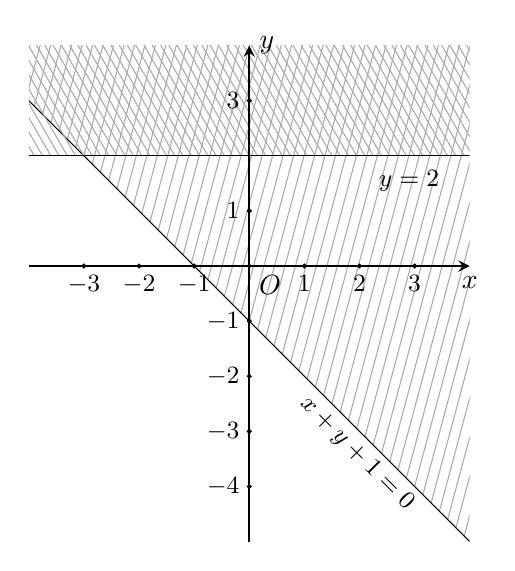
\begin{tikzpicture}[>=stealth,smooth,samples=100,scale=.7]
			\begin{scope}
				\clip (-4,-5) rectangle (4,4);
				%% Hàm thứ 1-----------------
				\pgfmathsetmacro{\goc}{-atan(1)+120}
				\foreach \i in {-12,-11.85,...,11}{
					\draw[gray!65,thin]({\i},{(-1*\i-1)/1})--+(\goc:15);}
				\draw plot[domain=-9:9]({\x},{(-1*\x-1)/1});
				\path (-1,0)--(1,-2) node[sloped,pos=1.7,shift={({\goc+150}:9pt)},font=\small]{$x+y+1=0$};
				%% Hàm thứ 2-----------------
				\pgfmathsetmacro{\goc}{-atan(0)+120}
				\foreach \i in {-12,-11.85,...,11}{
					\draw[gray!65,thin]({\i},{(-0*\i--2)/1})--+(\goc:15);}
				\draw plot[domain=-9:9]({\x},{(-0*\x--2)/1});
				\path (-1,2)--(1,2) node[sloped,pos=1.95,shift={({\goc+150}:9pt)},font=\small]{$y=2$};
			\end{scope}
			\draw[->,thick] (-4,0)--(4,0)node[below]{$x$};
			\draw[->,thick] (0,-5)--(0,4)node[right]{$y$};
			\draw[fill=black] (0,0) circle (1pt) node[below right]{$O$};
			\foreach \x in {
				-3,-2,-1,1,2,3
			}{
				\draw[fill=black] (\x,0)node[below]{\small $\x$} circle (1pt);
			}
			\foreach \y in {
				-4,-3,-2,-1,1,3
			}{
				\draw[fill=black] (0,\y)node[left]{\small $\y$} circle (1pt);
			}
		\end{tikzpicture}
	\end{center}
	}
\loigiai{
	- Vẽ hai đường thẳng $x+y+1=0$ và $y = 2$.\\
	- Biểu diễn miền nghiệm của từng bất phương trình trong hệ trên cùng một mặt phẳng tọa độ.\\
	Vậy miền nghiệm $D$ của hệ bất phương trình đã cho là miền không được tô (kể cả các đường biên).
	\begin{center}
		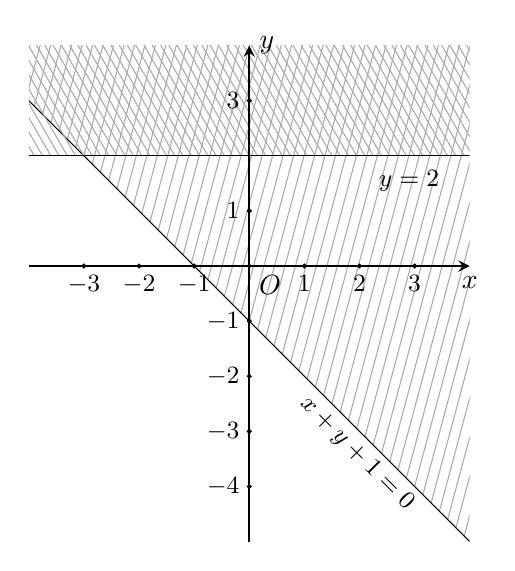
\begin{tikzpicture}[>=stealth,smooth,samples=100,scale=.7]
			\begin{scope}
				\clip (-4,-5) rectangle (4,4);
				%% Hàm thứ 1-----------------
				\pgfmathsetmacro{\goc}{-atan(1)+120}
				\foreach \i in {-12,-11.85,...,11}{
					\draw[gray!65,thin]({\i},{(-1*\i-1)/1})--+(\goc:15);}
				\draw plot[domain=-9:9]({\x},{(-1*\x-1)/1});
				\path (-1,0)--(1,-2) node[sloped,pos=1.7,shift={({\goc+150}:9pt)},font=\small]{$x+y+1=0$};
				%% Hàm thứ 2-----------------
				\pgfmathsetmacro{\goc}{-atan(0)+120}
				\foreach \i in {-12,-11.85,...,11}{
					\draw[gray!65,thin]({\i},{(-0*\i--2)/1})--+(\goc:15);}
				\draw plot[domain=-9:9]({\x},{(-0*\x--2)/1});
				\path (-1,2)--(1,2) node[sloped,pos=1.95,shift={({\goc+150}:9pt)},font=\small]{$y=2$};
			\end{scope}
			\draw[->,thick] (-4,0)--(4,0)node[below]{$x$};
			\draw[->,thick] (0,-5)--(0,4)node[right]{$y$};
			\draw[fill=black] (0,0) circle (1pt) node[below right]{$O$};
			\foreach \x in {
				-3,-2,-1,1,2,3
			}{
				\draw[fill=black] (\x,0)node[below]{\small $\x$} circle (1pt);
			}
			\foreach \y in {
				-4,-3,-2,-1,1,3
			}{
				\draw[fill=black] (0,\y)node[left]{\small $\y$} circle (1pt);
			}
		\end{tikzpicture}
	\end{center}
}
\end{bt}
\begin{bt}%[0T3B1-2]%[Dự án đề kiểm tra HKI NH22-23 - Quang Anh]%[Trường Chinh - Đề 4]
	Tìm tập xác định của hàm só: $y=\dfrac{\sqrt{x+3}}{\sqrt{2-x}}$. \dapso{$[-3;2)$}
		\loigiai{
		Điều kiện xác định của hàm số đã cho là
		$$ \heva{&x+3 \geq 0\\& 2-x>0} \Leftrightarrow \heva{&x \geq - 3 \\& x<2 } \Leftrightarrow x \in [-3;2). $$
		Vậy tập xác định của hàm số đã cho là $\mathscr{D} = [-3;2)$.
	}
\end{bt}
\begin{bt}%[0T3B2-2]%[Dự án đề kiểm tra HKI NH22-23 - Quang Anh]%[Trường Chinh - Đề 4]
	Xác định công thức của $P\colon y=2x^2+bx+c$, biết $(P)$ có đỉnh $I(-1; 3)$. \dapso{$b=4; c=5$}
		\loigiai{
		Vì đồ thị hàm số là một parabol có hoành độ đỉnh là $x_{I} = - \dfrac{b}{2a} \Leftrightarrow -1 = -\dfrac{b}{4} \Rightarrow b = 4$. $\hfill (1)$\\
		Đồ thị hàm số đi qua điểm $I(-1; 3)$ nên $3 =2\cdot (-1)^2 + b\cdot (-1) + c \Leftrightarrow -b + c = 1$. $\hfill (2)$\\
		Từ $(1)$ và $(2)$, ta có hệ phương trình
		$$ \heva{&b = 4\\& -b + c = 1} \Leftrightarrow \heva{&b = 4\\&c = 5.} $$
		Vậy $y = 2x^2 + 4x + 5$.
	}
\end{bt}
\begin{bt}%[0T6B4-1]%[Dự án đề kiểm tra HKI NH22-23 - Quang Anh]%[Trường Chinh - Đề 4]
	Một cửa hàng trà sữa vừa khai trương, thống kê lượng khách tới quán trong 7 ngày đầu và thu được mẩu số liệu sau:
	\begin{center}
		\begin{tabular}{|c|c|c|c|c|c|c|}
			\hline \text { Ngày 1 } & \text { Ngày 2 } & \text { Ngày } 3 & \text { Ngày } 4 & \text { Ngày 5 } & \text { Ngày 6 } & \text { Ngày } 7 \\
			\hline 575 & 454 & 400 & 325 & 351 & 333 & 412 \\
			\hline
		\end{tabular}
	\end{center}
	Tìm số trung bình, trung vị, khoảng biến thiên và khoảng tứ phân vị của mẫu số liệu.
	\dapso{$\overline{x}\approx 407{,}14$; $M_e=400$; $R=250$; $\Delta_Q=121$}
		\loigiai{
		- Số trung bình là
		$$ \bar{x} = \dfrac{1}{7}(325 + 333 + 351 + 400 + 412 + 454 + 575) = 407{,}14. $$
		Sắp xếp lại mẫu số liệu theo thứ tự không giảm, ta được
		$$ 325; 333; 351; 400; 412; 454; 575. $$
		- Khoảng biến thiên của mẫu số liệu là $R = 575 - 325 = 250$.\\
		- Cỡ mẫu là $n = 7$ là số lẻ nên giá trị phân vị thứ hai là $M_e = Q_2 = 400$.\\
		- Tứ phân vị thứ nhất là trung vị của mẫu $325; 333; 351$. Do đó, $Q_1 = 333$.\\
		- Tứ phân vị thứ ba là trung vị của mẫu $412; 454; 575$. Do đó, $Q_3 = 454$.\\
		- Khoảng tứ phân vị của mẫu số liệu $
		\Delta_Q=Q_3-Q_1=454-333=121$.
	}
\end{bt}
\begin{bt}%[0T4B2-1]%[Dự án đề kiểm tra HKI NH22-23 - Quang Anh]%[Trường Chinh - Đề 4]
	Cho tam giác $ABC$ có $AB=2, BC=3, AC=4$. Tính số đo góc $B$, tính diện tích, bán kính đường tròn ngoại tiếp và đường cao $AH$ của tam giác $ABC$.
	\dapso{$\widehat{B}\approx 104^\circ 29', S=\dfrac{3\sqrt{15}}{4}, R=\dfrac{8\sqrt{15}}{15}, AH=\dfrac{3\sqrt{15}}{8}$}
	\loigiai{
			\begin{center}
				\begin{tikzpicture}[>=stealth,line join=round,line cap=round,font=\footnotesize,scale=1]
					\path
					(1.7,2) coordinate (B)
					(0,0) coordinate (A)
					(5,0) coordinate (C);
					\draw (A)--(B)--(C)--(A);
					\fill ($(A)!0.5!(B)$) node[shift={(120:3mm)}]{$2$};
					\fill ($(A)!0.5!(C)$) node[shift={(-60:3mm)}]{$4$};
					\fill ($(B)!0.5!(C)$) node[shift={(90:3mm)}]{$3$};
					\foreach \p/\r in {B/90,A/-135,C/-45}
					\fill (\p) circle (1.2pt) node[shift={(\r:3mm)}]{$\p$};
				\end{tikzpicture}
			\end{center}
			Xét tam giác $ABC$, áp dụng hệ quả của định lí cosin, ta có
			$$ \cos B = \dfrac{a^2 + c^2 - b^2}{2ac} = \dfrac{2^2 + 3^2 - 4^2}{2\cdot 2\cdot 3} = -\dfrac{1}{4} \Rightarrow \widehat{B} \approx 104^\circ 29'. $$
			Vì $\widehat{B} \approx 104^\circ29'$ là góc lẻ nên ta sẽ dùng công thức Hê - rông để tính diện tích.\\
			Nửa chu vi của tam giác $ABC$ là $p = \dfrac{a + b +c}{2} = \dfrac{2 + 4 + 3}{2} = 4{,}5$.\\
			Do đó, diện tích tam giác $ABC$ là
			$$ S_{\triangle ABC} = \sqrt{p(p-a)(p-b)(p-c)} = \dfrac{3\sqrt{15}}{4}. $$
			Mặt khác, ta có $S_{\triangle ABC} = \dfrac{1}{2}AH\cdot BC \Rightarrow AH = \dfrac{2S_{\triangle ABC}}{BC} = \dfrac{\sqrt{15}}{2}$.\\
			Ta cũng có $S_{\triangle ABC} = \dfrac{abc}{4R} \Rightarrow  R = \dfrac{abc}{4S_{\triangle ABC}} =\dfrac{8\sqrt{15}}{15}$.
		}
\end{bt}
\begin{bt}%[0T5B2-2]%[0T5B4-1]%[Dự án đề kiểm tra HKI NH22-23 - Quang Anh]%[Trường Chinh - Đề 4]
	Cho tam giác $ABC$. Gọi $K, H$ lần lượt là trung điểm $BC, AK$. Điểm $M$ tùy ý.
	\begin{enumerate}
		\item Chứng minh rằng: $\vec{AM}+\vec{BC}=\vec{AC}+\vec{BM}$.
		\item Chứng minh rằng: $2\vec{MA}+\vec{MB}+\vec{MC}=4 \vec{MH}$.
		\item Tính $\vec{BC} \cdot \vec{BK}$ biết $BC=8$. \dapso{$32$}
	\end{enumerate}	
  \loigiai{
	\begin{enumerate}
		\item Ta có $\vec{AM}+\vec{BC}= \overrightarrow{AB} + \overrightarrow{BM} + \overrightarrow{BA} + \overrightarrow{AC} = \vec{AC}+\vec{BM} + \overrightarrow{AB} + \overrightarrow{BA} = \vec{AC}+\vec{BM}$.
		\item Ta có $\begin{aligned}[t]
			VT = 2\vec{MA}+\vec{MB}+\vec{MC}
			= 2\vec{MA}+2\vec{MK}
			= 2(\vec{MA}+\vec{MK})=2\cdot2\vec{MH}=4\vec{MH}=VP.
		\end{aligned}$\\
		Vậy $2\vec{MA}+\vec{MB}+\vec{MC}=4 \vec{MH}$.
		\item Ta có $BC = 8$, $BK = \dfrac{BC}{2} = 4$, $\overrightarrow{BC}$ cùng hướng với $\overrightarrow{BK}$.\\
		Suy ra,
		$$ \overrightarrow{BC}\cdot\overrightarrow{BK} = \left| \overrightarrow{BC}\right|\cdot\left|\overrightarrow{BK} \right|\cdot \cos{0^\circ} = 8\cdot 4\cdot 1= 32. $$
	\end{enumerate}
}
\end{bt}
\begin{bt}%[0T5T4-1]%[0T4T2-1]%[0T2K2-2]%[Dự án đề kiểm tra HKI NH22-23 - Quang Anh]%[Trường Chinh - Đề 4]
	\begin{enumerate}
		\item Một người dùng một lực $\vec{F}$ có cường độ $30 \mathrm{~N}$ kéo một chiếc xe đi quãng đường đài $60 \mathrm{~m}$. Tính công sinh bởi lực $\vec{F}$, biết rằng góc giữa vectơ $\vec{F}$ và hướng di chuyển là $45^{\circ}$. \dapso{$900\sqrt{2}$ J}
		\item
		\immini{
			Giả sử $CD=h$ là chiều cao của tháp trong đó $C$ là chân tháp. Chọn hai điểm $A, B$ trên mặt đất sao cho ba điểm $A, B, C$ thẳng hàng. Ta đo được $AB=24$ m, $\widehat{CAD}=63^{\circ}$; $\widehat{CBD}=48^{\circ}$. Tính chiều cao $h$ của khối tháp?
			\dapso{$h\approx 61{,}4$ m}
		}{
			\begin{tikzpicture}[scale=1, font=\footnotesize, line join=round, line cap=round,>=stealth]
				\def\gn{48}
				\def\gl{63}
				\def\h{3.5}
				\pgfmathsetmacro{\x}{
					\h/ tan(\gn)
				};
				\pgfmathsetmacro{\g}{
					\h/ tan(\gl)
				};
				\path		
				(\g,0) coordinate (G)
				(\x,0) coordinate (X)
				(0,\h) coordinate (T)
				(0,0) coordinate (B)
				;
				\draw [fill=red!30]
				(-.3,0)
				.. controls ++(50:0.5) and ++(265: 1) .. (T) 
				.. controls ++(-85:1) and ++(130: 0.5) .. (.3,0)--cycle;
				\draw (G)--(B)--(T)--(G)--(X)node[pos=0.5,below]{$24\,\text{m}$}--(B) (T)--(X);
				\foreach \x/\g/\n in{G/-90/A,X/-60/B, T/90/D, B/-90/C}
				\fill[black] (\x) circle (1pt)+(\g:3mm) node {$\n$};
				\draw 
				pic[draw, angle radius=2mm]{angle=T--X--B}
				pic[draw, angle radius=2.5mm]{angle=T--X--B}; 
				\draw pic[draw, angle radius=2mm]{angle=T--G--B};
				\path 
				(X)+(162:5mm)node{$48^\circ$}
				(G)+(155:4mm)node{$63^\circ$};
			\end{tikzpicture}
		} 
		\item Trong một cuộc thi pha chế, mỗi đội chơi được sử dụng tối đa $24 \mathrm{~g}$ hương liệu, 9 lít nước và $210 \mathrm{~g}$ đường để pha chế nước cam và nước táo. Để pha chế 1 lít nước cam cần $30 \mathrm{~g}$ đường, 1 lít nước và $1 \mathrm{~g}$ hương liệu, pha chế 1 lít nước táo cần $10 \mathrm{~g}$ đường, 1 lít nước và $4 \mathrm{~g}$ hương liệu. Mỗi lít nước cam nhận được 60 điểm thưởng, Mỗi lít nước táo nhận được 80 điểm thưởng. Hỏi cần pha chế bao nhiêu lít nước trái cây mỗi loại để số điểm thưởng là lớn nhất. \dapso{$4$ lít nước cam và $5$ lít nước táo}
	\end{enumerate}	
\loigiai{
	\begin{enumerate}
		\item Công sinh bởi lực $\overrightarrow{F}$ là
		$$ \overrightarrow{F}\cdot \overrightarrow{d} = \left|\overrightarrow{F} \right|\cdot \left|\overrightarrow{d} \right|\cdot \cos 45^\circ = 30\cdot 60\cdot \dfrac{\sqrt{2}}{2} = 900\sqrt{2} \quad \textrm{(J).}$$
		\item \immini{$\triangle DCA$ vuông tại $C$ nên $\tan 63^\circ =\dfrac{DC}{AC}\\ \Rightarrow AC=\dfrac{DC}{\tan 63^\circ}=\dfrac{h}{\tan 63^\circ}$ m.\\
			$\triangle DCB$ vuông tại $C$ nên $\tan 48^\circ =\dfrac{DC}{BC}\\\Rightarrow BC=\dfrac{DC}{\tan 48^\circ}=\dfrac{h}{\tan 48^\circ}$ m.\\
			Mà $BC-AC=24\Leftrightarrow \dfrac{h}{\tan 48^\circ}-\dfrac{h}{\tan 63^\circ}=24 \\ \Leftrightarrow h=24:\left(\dfrac{1}{\tan 48^\circ}-\dfrac{1}{\tan 63^\circ}\right)\approx 61{,}4$ m.}
		{	\begin{tikzpicture}[scale=1, font=\footnotesize, line join=round, line cap=round,>=stealth]
				\def\gn{48}
				\def\gl{63}
				\def\h{3.5}
				\pgfmathsetmacro{\x}{
					\h/ tan(\gn)
				};
				\pgfmathsetmacro{\g}{
					\h/ tan(\gl)
				};
				\path		
				(\g,0) coordinate (G)
				(\x,0) coordinate (X)
				(0,\h) coordinate (T)
				(0,0) coordinate (B)
				;
				\draw [fill=red!30]
				(-.3,0)
				.. controls ++(50:0.5) and ++(265: 1) .. (T) 
				.. controls ++(-85:1) and ++(130: 0.5) .. (.3,0)--cycle;
				\draw (G)--(B)--(T)--(G)--(X)node[pos=0.5,below]{$24\,\text{m}$}--(B) (T)--(X);
				\foreach \x/\g/\n in{G/-90/A,X/-60/B, T/90/D, B/-90/C}
				\fill[black] (\x) circle (1pt)+(\g:3mm) node {$\n$};
				\draw 
				pic[draw, angle radius=2mm]{angle=T--X--B}
				pic[draw, angle radius=2.5mm]{angle=T--X--B}; 
				\draw pic[draw, angle radius=2mm]{angle=T--G--B};
				\path 
				(X)+(162:5mm)node{$48^\circ$}
				(G)+(155:4mm)node{$63^\circ$};
			\end{tikzpicture}
	} 
		\item Gọi $x$ và $y$ (lít) lần lượt là số lít nước cam và nước táo cần pha chế $(x,y \geq 0)$. $\hfill (1)$\\
		Số gam hương liệu cần để pha được $x$ lít nước cam và $y$ lít nước táo là $x + 4y$.\\ Mà người này chỉ có $24$ gam hương liệu nên $x + 4y \leq 24$. $\hfill(2)$\\
		Số lít nước cần để pha được $x$ lít nước cam và $y$ lít nước táo là $x + y$.\\ Mà người này chỉ có $9$ lít nước nên $x + y \leq 9$. $\hfill(3)$\\
		Số gam đường cần để pha được $x$ lít nước cam và $y$ lít nước táo là $30x + 10y$.\\ Mà người này chỉ có $210$ gam đường nên $30x + 10y \leq 210$. $\hfill(4)$\\
		Từ $(1)$, $(2)$, $(3)$, $(4)$ ta có hệ bất phương trình
		$$ \heva{&x \geq 0\\&y \geq 0\\&x + 4y \leq 24\\&x + y \leq 9\\&30x + 10y \leq 210.} \quad (*) $$
		Vì mỗi lít nước cam nhận được 60 điểm thưởng, mỗi lít nước táo nhận được 80 điểm thưởng nên số điểm thưởng khi pha chế $x$ lít nước cam và $y$ lít nước táo là $T(x;y) = 60x + 80y$ (điểm).\\
		Biểu diễn miền nghiệm của hệ bất phương trình $(*)$ (là phần bị gạch chéo có tính cả các đường biên) như sau.
		\begin{center}
			\begin{tikzpicture}[>=stealth,line join=round,line cap=round,font=\footnotesize,scale=1]
				\draw[->,line width = 1pt] (-0.5,0)--(0,0) node[below left]{$O$}--(5.5,0) node[below]{$x$};
				\draw[->,line width = 1pt] (0,-0.5) --(0,5) node[right]{$y$};
				\fill (0,1.2) node[left,scale = 0.7]{$6$} circle (1pt);
				\fill (0,1.8) node[left,scale = 0.7]{$9$} circle (1pt);
				\fill (0,4.2) node[left,scale = 0.7]{$21$} circle (1pt);
				\fill (1.4,0) node[below,scale = 0.7]{$7$} circle (1pt);
				\fill (1.8,0) node[below,scale = 0.7]{$9$} circle (1pt);
				\fill (4.8,0) node[below,scale = 0.7]{$24$} circle (1pt);
				\fill (1.2,0.6) circle (1pt);
				\fill (0.8,1) circle (1pt);
				\draw (0,1.2)--(4.8,0) (0,1.8)--(1.8,0) (0,4.2)--(1.4,0);
				\fill[opacity=.2,pattern= vertical lines] (0,0)--(0,1.2)--(0.8,1)--(1.2,0.6)--(1.4,0)--cycle;
			\end{tikzpicture}
		\end{center}
		Miền nghiệm của hệ $(*)$ là một đa giác có các đỉnh có tọa độ là $(0;0)$, $(0;6)$, $(4;5)$, $(6;3)$, $(7;0)$. Tính toán $T(x;y)$ tại các đỉnh này ta có $T(4;5) = 640$ (điểm) là lớn nhất.\\
		Vậy đội chơi cần pha $4$ lít nước cam và $5$ lít nước táo để có điểm thưởng lớn nhất.
	\end{enumerate}
	
}
\end{bt}








